%----------------------------------------------------------------------------------------
%	EISCAT MADRIGAL.
%----------------------------------------------------------------------------------------

\section{EISCAT Madrigal}
In figure \ref{fig:madrigal} the EISCAT data from the 30th of October 2003 is shown. There are a few white gaps which can be explained by interference like clouds in the atmosphere. On top we have the electron density, followed by the electron temperature, ion temperature, ion drift velocity and the system temperature. \\

Around 20:50 on the 29th of October 2003, one of the main peaks during this solar storm was measured. When this peak was over there was a dip in electron density, as can be seen from figure \ref{fig:madrigal}. Then, on the 30th of October there were some M-flares at 1:55 till 2:45 and 15:20 till 15:40 measured by GOES \cite{goes_x-ray_archive}. You can see in the EISCAT data that right after this change has been measured the densities and temperatures started increasing. The peaks are delayed by a a couple of hours in this data. \\

When comparing the data from the 30th of October 2003 to a more quit day, like the one in figure \ref{fig::resultsE1}, it can be seen that especially the fluctuations are way more intense. The gradient between upper and lower in the atmosphere is still present. But everything is, on average, more intense. The perturbations go deeper into the atmosphere and with higher velocities.





\begin{figure}
\centering
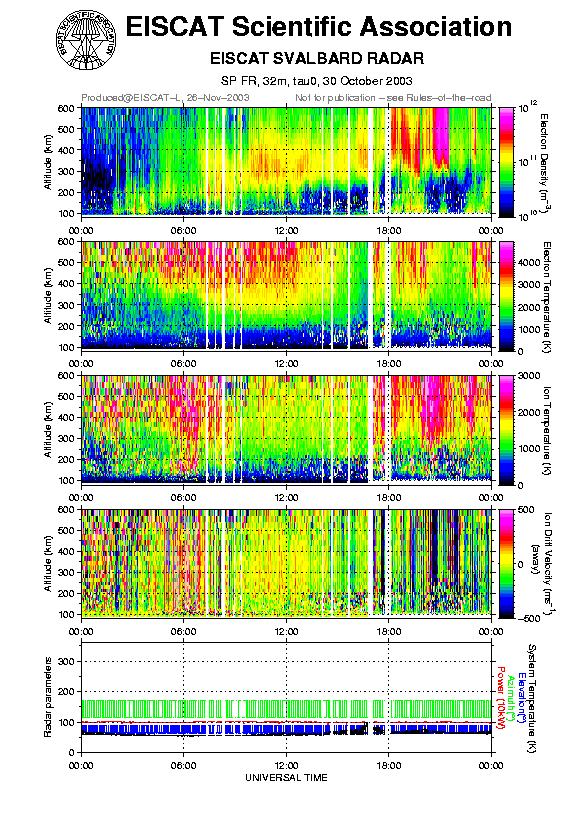
\includegraphics[width=.9\textwidth]{figures/2003-10-30_SvalvardPlot.png}
\caption{EISCAT radar data from the upper atmosphere science database Madrigal \cite{madrigal}.}
\label{fig:madrigal}
\end{figure}